\documentclass{article}
\usepackage[utf8]{inputenc}
\pagenumbering{Roman}
\usepackage{ragged2e}
\usepackage{graphicx}
\usepackage{wrapfig}
\usepackage[spanish]{babel}
\usepackage{hyperref}
\usepackage{datetime}


\begin{document}


\title{\huge \textbf{Instructivo para la extracción de datos de monitor de signos vitales y BIS } \vspace{8cm}}
\author{Carlos Valle \\ \href{mailto:cgvalle@uc.cl}{cgvalle@uc.cl} }
\date{21 de Febrero 2024}
\maketitle


\newpage

\section{Motivación}

El objetivo de este manual es orientar en la configuración de equipos y software necesarios para la extracción de datos de dos dispositivos: el monitor de signos vitales \href{https://www.gehealthcare.com/products/patient-monitoring/patient-monitors/carescape-monitor-b650}{Carescape B650} y el monitor \href{https://www.medtronic.com/covidien/es-cl/products/brain-monitoring/bis-complete-4-channel-monitor.html}{Bis vista}.

Dado que los procesos para recolectar datos de cada equipo son independientes, se dividirán en dos secciones separadas dentro de este documento. A pesar de esta independencia, se aconseja enfocarse en un dispositivo a la vez para una mayor eficacia. En cada sección, se detallará tanto la configuración inicial como el manejo del software correspondiente.

Para acceder a los códigos y archivos necesarios para este procedimiento, visite la carpeta de GitHub en el siguiente enlace: \url{https://github.com/cgvalle/monitor_signos_vitales}.




\newpage



% B650
\section{Monitor Carescape B650}
Para la extracción de las señales fisiológicas durante cirugia se utiliza el monitor Carescape B650 (Fig. \ref{fig:b650_frontal}). Los códigos e instructivos se basan en dicho monitor, por lo que no se asegura la compatibilidad con un tercero. 

\begin{figure}[h]
	\centering
    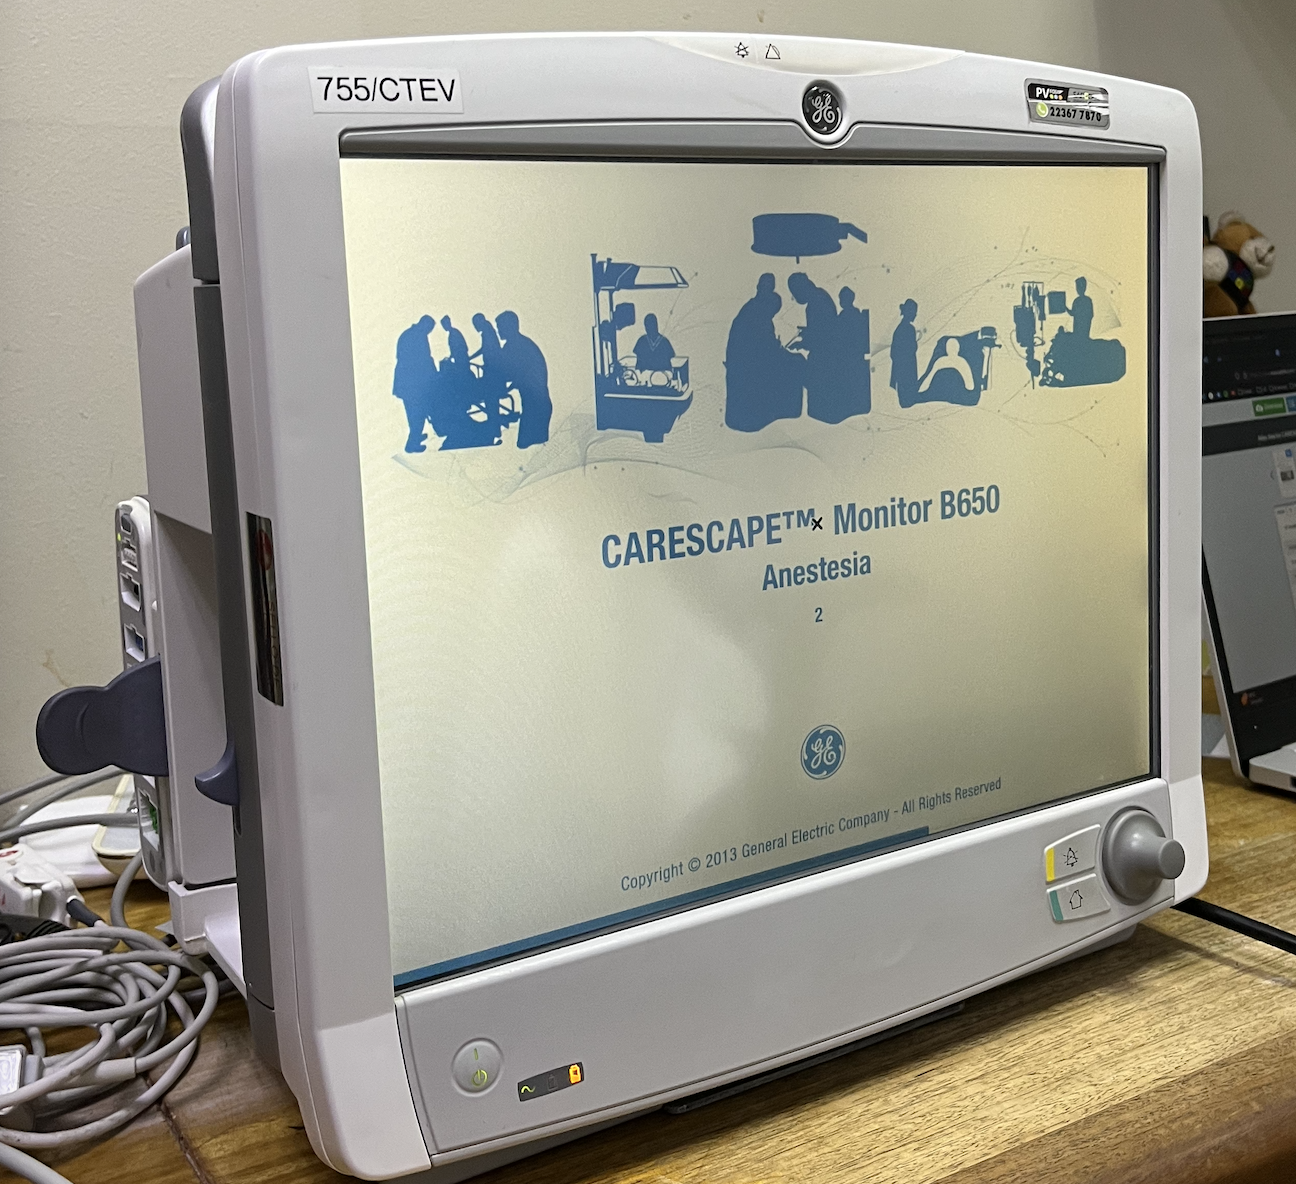
\includegraphics[scale=0.6]{img/carescape_b650.jpeg}
    \caption{Vista frontal monitor Carescape B650}
    \label{fig:b650_frontal}
\end{figure}

\subsection{Preparativos}
Antes de comenzar es necesario configurar el monitor para que envíe los datos a un computador, cambiando la configuración de red (Network Type) a S/5 Collect. Para esto se debe seguir el siguiente procedimiento:

\begin{enumerate}
	\item Encender el monitor y esperar a que cargue.
	\item Ir a la pantalla de Config. Monitor y seleccionar configuración. 
	\item Se le solicitara un usuario y contraseña. Los valores por defecto son: para usuario \textbf{biomed} y la contraseña es \textbf{Change Me}. Si no funcionan, contactar al servicio TI del hospital para obtener las credenciales.
	\item Una vez dentro de la configuración, seleccionar la pestaña de red y cambiar el Network Type a S/5 (Fig. \ref{fig:network_type}). Luego dar click en next
	
	\begin{figure}[h]
		\centering
		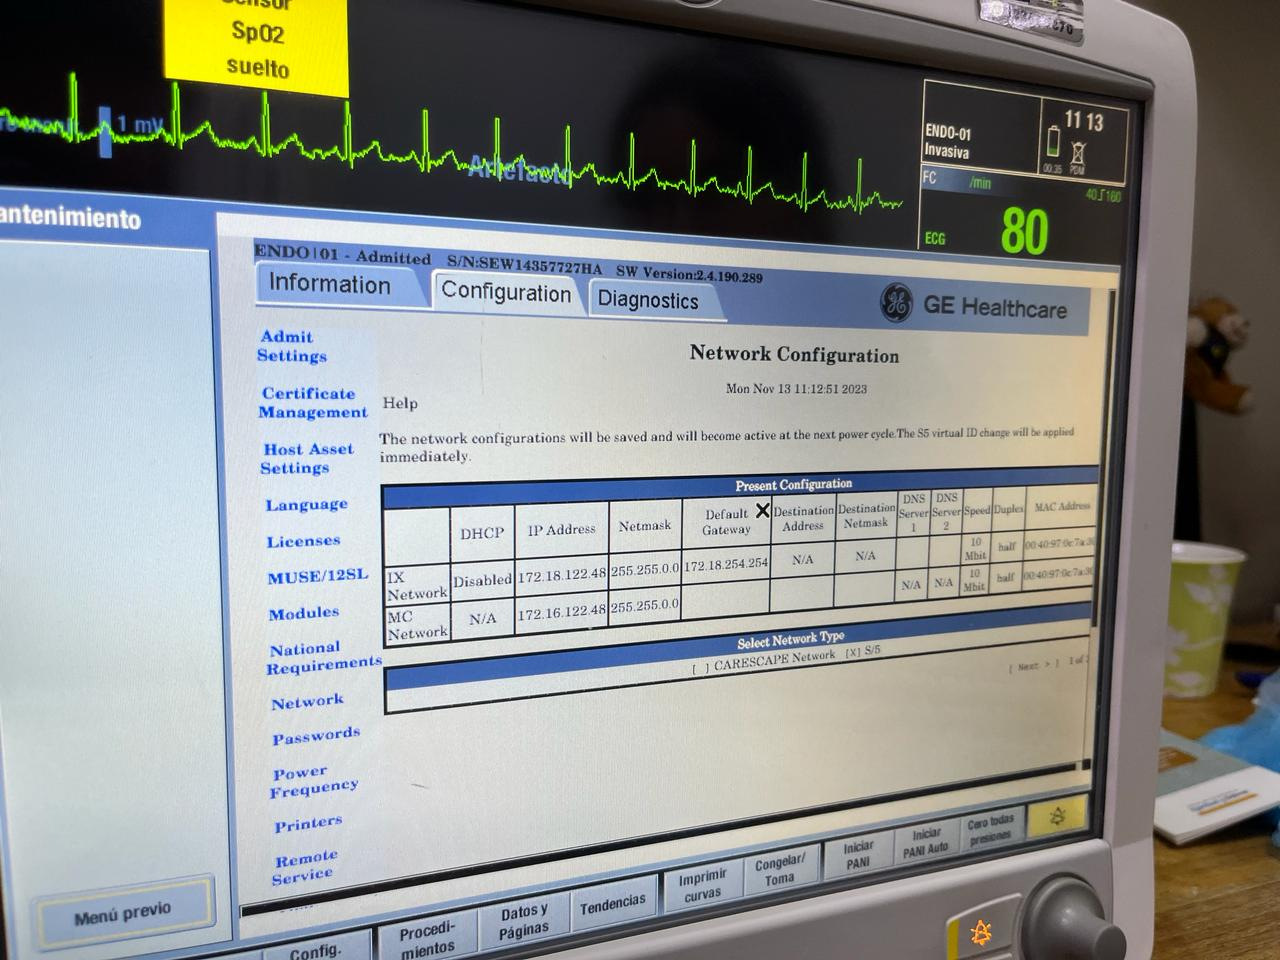
\includegraphics[scale=0.3]{img/network.png}
		\caption{Red configurada en S/5}
		\label{fig:network_type}
	\end{figure}

	\item En el apartado de Virtual ID utilizar el numero 50001 o mayor (Fig. \ref{fig:virtual_id}). 
	
	\begin{figure}[h]
		\centering
		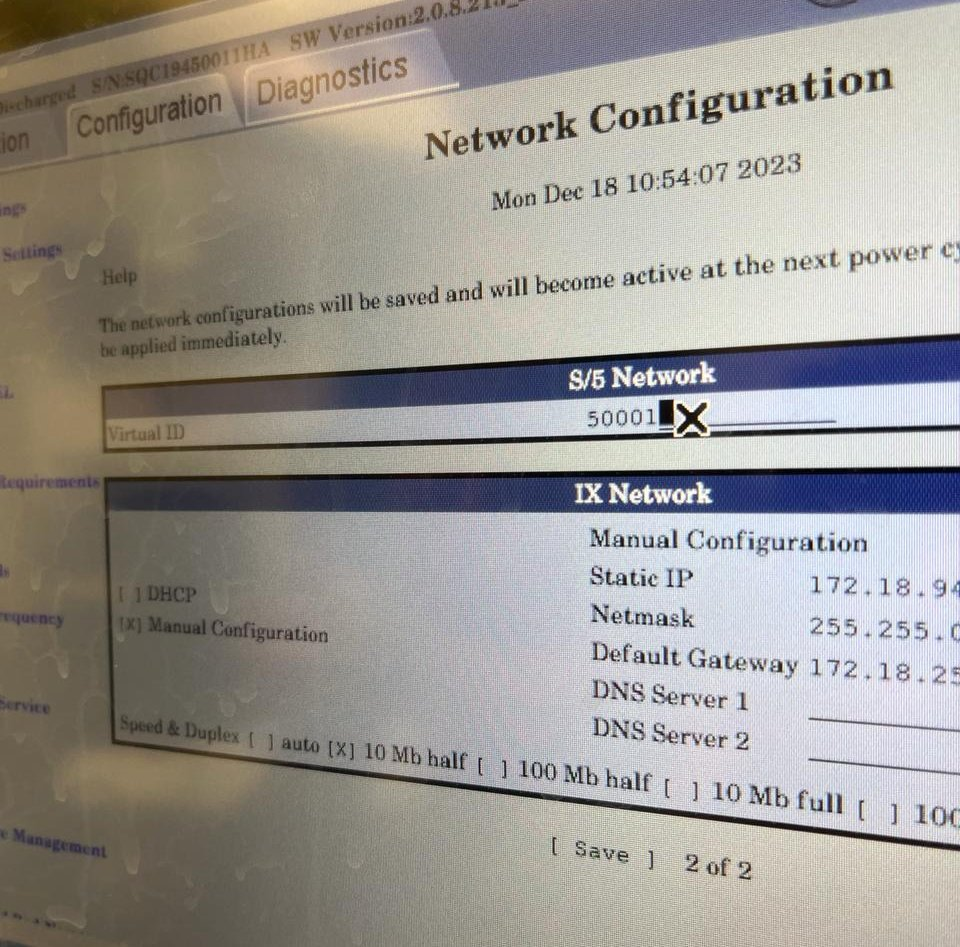
\includegraphics[scale=0.3]{img/network_id.jpeg}
		\caption{Virtual ID}
		\label{fig:virtual_id}
	\end{figure}
	\item Guardar los cambios y reiniciar el monitor.
	\item Cambiar fecha y hora del monitor, para que coincida con la del computador al que se conectará incluidos los segundos.

\end{enumerate}

Es importante hacer notas que este proceso puede variar dependiendo de la versión del software del monitor, pero en general el proceso es similar aunque con variaciones en la interfas. 






\subsection{Setup}
Cables necesarios:

\begin{enumerate}
	\item Cable ATEN USB to Serial RS232.  (Es necesario que cuente con el chip VID 0557, modelos mas nuevos vienen con 067b. De necesitar otro, buscarlo en ebay priorizando el más viejo que exista para aumentar las probabilidades de que venga con el chip VID 0557)

	\includegraphics*[scale=0.12]{img/ATEN_USB.jpeg}
	\item  Cable RS232 hembra hembra 

	\includegraphics*[scale=0.12]{img/rs232_hembra_hembra.jpeg}
	\item Cable RS232 a usb (Null Modem)

	\includegraphics*[scale=0.12]{img/rs232_macho_a_usb.jpeg}

\end{enumerate}

Se conectan los 3 cables en serie, quedando con dos extremos USB. El USB del cable 3 se conecta al computador y el USB del cable 1 se conecta al monitor. Es necesario que este utilmo se conecte al monitor mediante la entrada USB inferior derecha, tal como se ve en la imagen.

\begin{figure}[h]
	\centering
	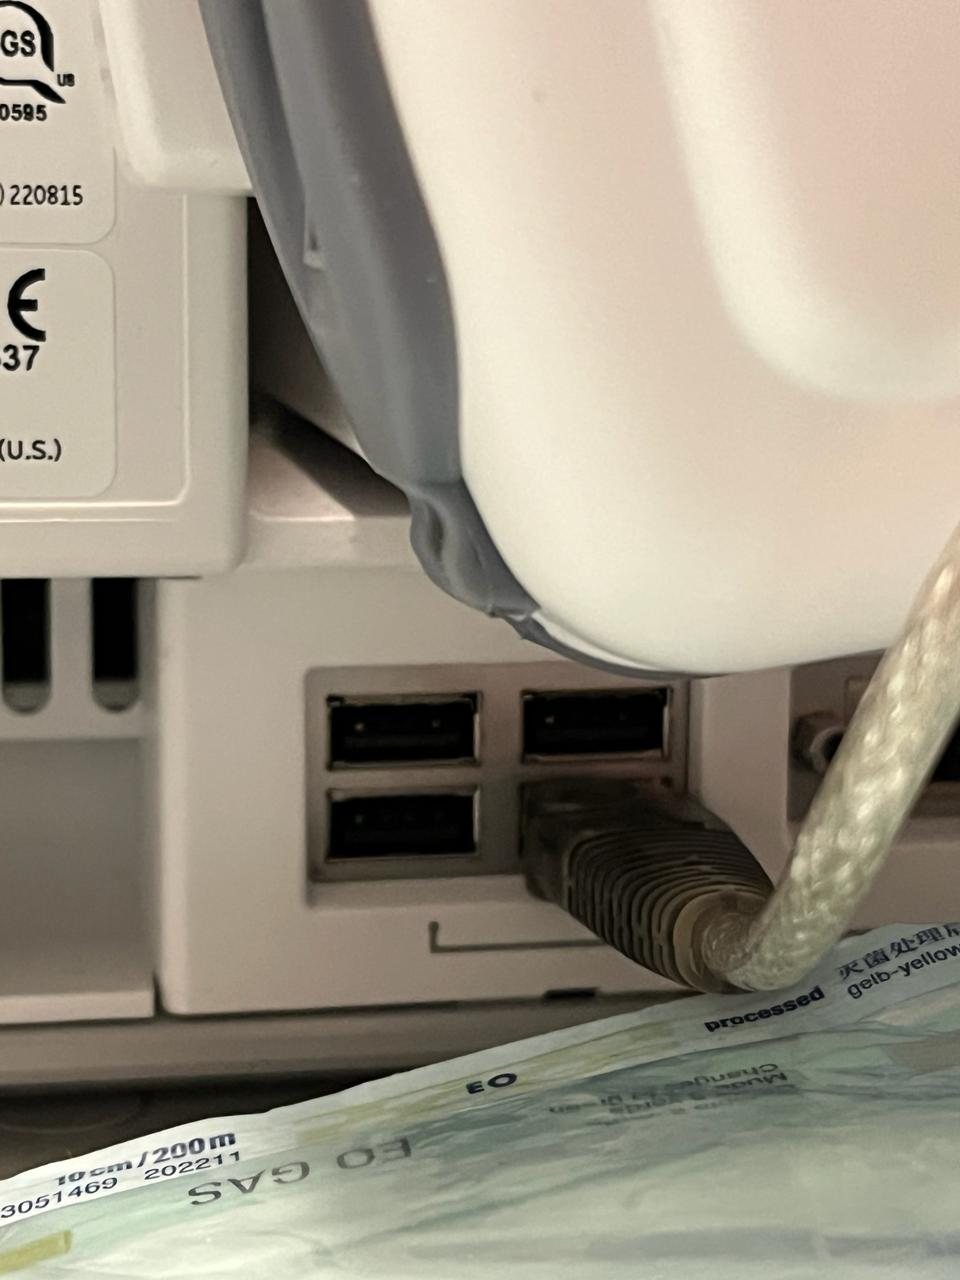
\includegraphics[scale=0.2]{img/b650_rear_panel.png}
	\caption{Vista posterior monitor Carescape B650. Solo se debe usar el usb inferior derecho.}
	\label{fig:b650_posterior}
\end{figure}

El otro extremo, puede ir conectado a cualquier puerto USB del computador.



\subsection{Uso}
Clonar el repositorio de Github: \url{https://github.com/cgvalle/monitor_signos_vitales}. En la carpeta \textbf{monitor\_record} encontraras dos archivos:
\begin{itemize}
	\item \textbf{VSCapture.exe}: Este programa se encarga de capturar los datos del monitor y guardarlos en un archivo .csv.
	\item \textbf{README.md}: Instructivo rapido de uso.
\end{itemize}

Una vez iniciado VSCapture, deberá ingresar el puerto COM al cual está conectado el monitor. Si solo hay un dispositivo conectado, el puerto COM a utilizar será el que se muestra automáticamente en la lista. En caso contrario, será necesario buscarlo manualmente en el Administrador de Dispositivos de Windows. A continuación, debe seleccionar el intervalo de transmisión de datos, para lo cual se recomienda un valor de 1 segundo. Por último, se le solicitará que elija el tipo de datos que desea capturar, teniendo a su disposición 5 opciones diferentes. Este proceso se ilustra en la Figura \ref{fig:vs_capture}.


\begin{figure}[h]
	\centering
	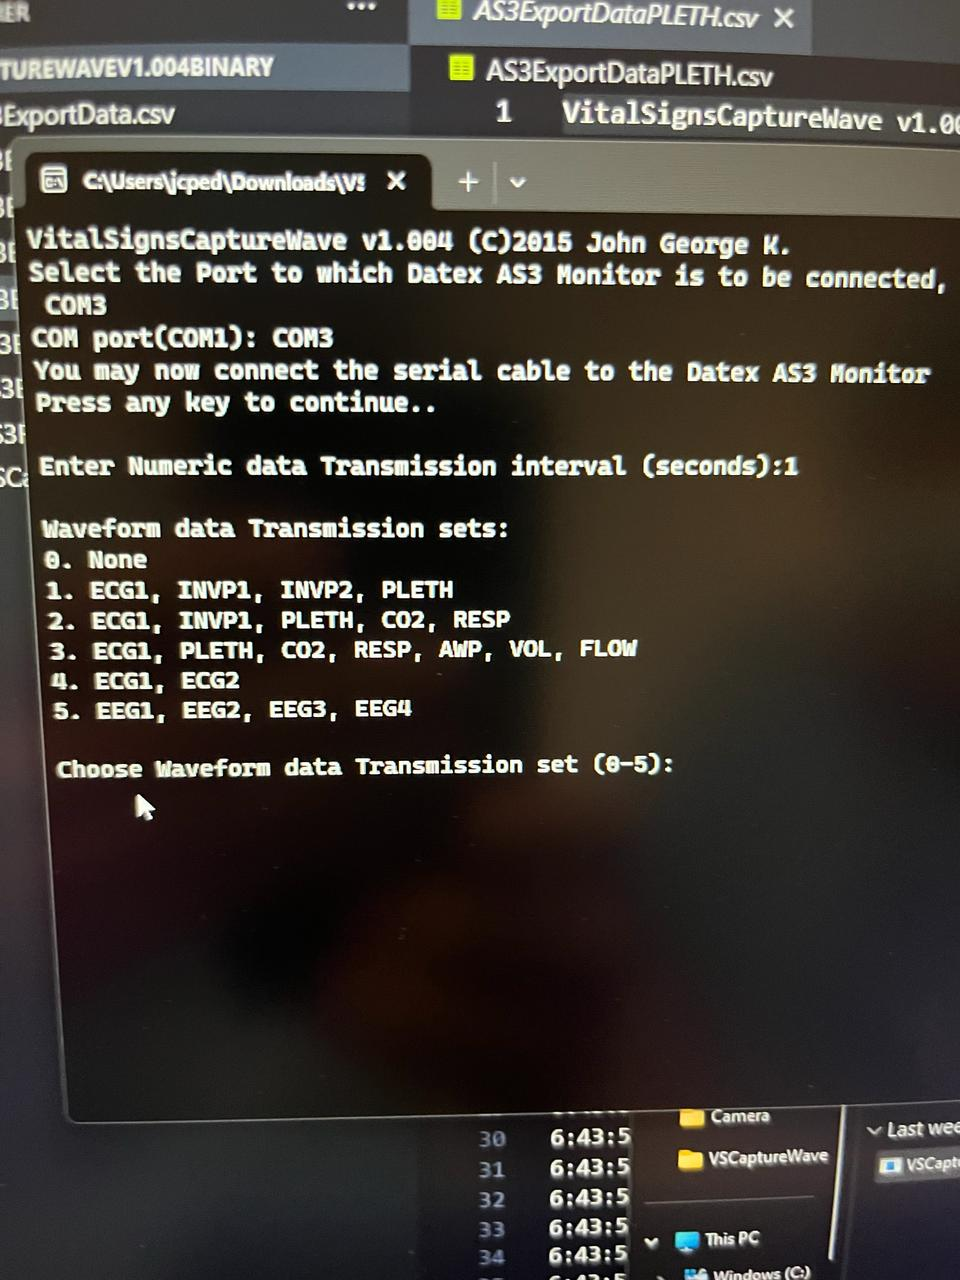
\includegraphics[scale=0.2]{img/vs_capture.png}
	\caption{Proceso de captura de datos con VSCapture.}
	\label{fig:vs_capture}
\end{figure}



Al seleccionar el tipo de datos, es importante asegurarse de que los canales seleccionados sean aquellos que se están utilizando en la cirugía. En particular, las líneas invasivas de presión arterial disponen de múltiples canales; por ello, se recomienda siempre conectarlas al canal 1. Si se conectan al canal 2, no se obtendrán datos con la opción 2 de VSCapture, dado que esta solo captura el canal 1 (INVP1), como se muestra en la Figura \ref{fig:canal}.


\begin{figure}[h]
	\centering
	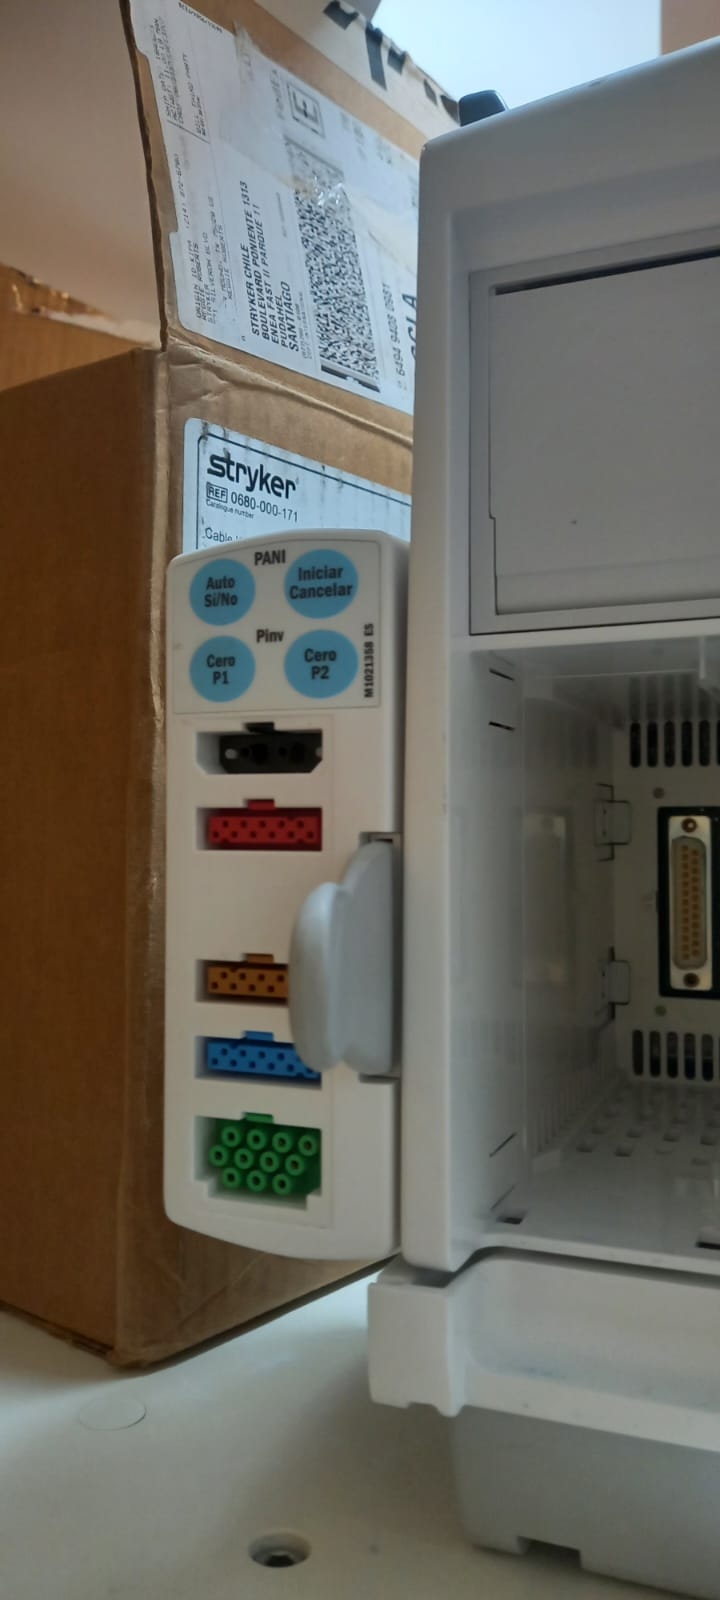
\includegraphics[scale=0.2]{img/canal.png}
	\caption{Verificar que se este utilizando el canal correcto. Los puertos pueden variar dependiendo del monitor incluso dentro de la familia B650.}
	\label{fig:canal}
\end{figure}




Al finalizar la cirugia, se debe presionar el botón de ESCAPE en la terminal del programa para que se terminar con la adquisición. Este archivo se guardara en la carpeta \textbf{monitor\_record} con el nombre de \textbf{*.csv}.


\newpage

\subsection{Resolución de problemas}

\begin{itemize}
	\item Si el programa se congela o no responde, se recomienda reinicar programa. Verificar que las conexiones esten bien hechas y que el puerto COM seleccionado sea el correcto. Se recomienda utilizar cinta adhesiva para asegurar que los cables no se desconecten.
	\item Si el monitor no envia datos, verificar que el Network Type este configurado en S/5 y que el Virtual ID sea el correcto.
	\item Si el monitor no envia datos, verificar que el puerto COM seleccionado sea el correcto.
	\item Si el monitor no envia datos, verificar que el cable USB a RS232 este conectado al puerto USB inferior derecho del monitor.
\end{itemize}



\section{Monitor BIS Vista}

El monitor BIS Vista (Fig. \ref{fig:bis_frontal}) es un monitor de electroencefalografía que se utiliza para medir el nivel de conciencia del paciente. 

\begin{figure}[h]
	\centering
	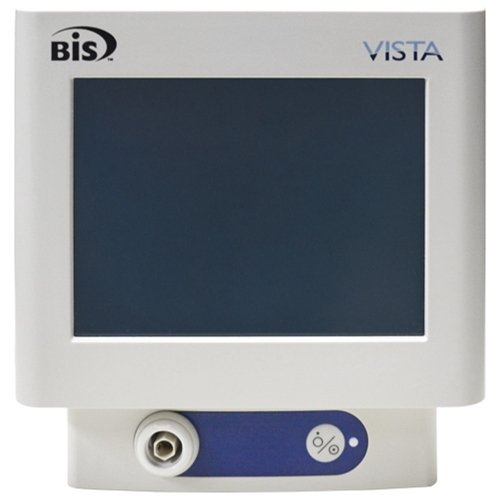
\includegraphics[scale=0.2]{img/bis_vista.png}
	\caption{Vista frontal monitor BIS Vista}
	\label{fig:bis_frontal}
\end{figure}



\subsection{Preparativos}
De forma similar al monitor Carescape B650, es necesario configurar la hora y la fecha en el monitor a través del botón 'Fecha y hora' en el menú del equipo, para asegurar que coincida con la del computador al cual se conectará. Es crucial realizar este paso correctamente para evitar discrepancias en los datos.

\subsection{Setup}

Elementos necesarios:

\begin{enumerate}
	\item Cable RS232 macho a usb (se recomienda el modelo Trendnet TU-S9)
	\item Cable RS232 macho hembra
	\item Pendrive USB 
\end{enumerate}

Se conectan ambos cables en serie, quedando con un extremo USB. El USB del cable se conecta al computador y el otro extremo se conecta al monitor. El pendrive se conecta al puerto USB del monitor (Fig. \ref{fig:bis_rear_panel}).


\begin{figure}
	\centering
    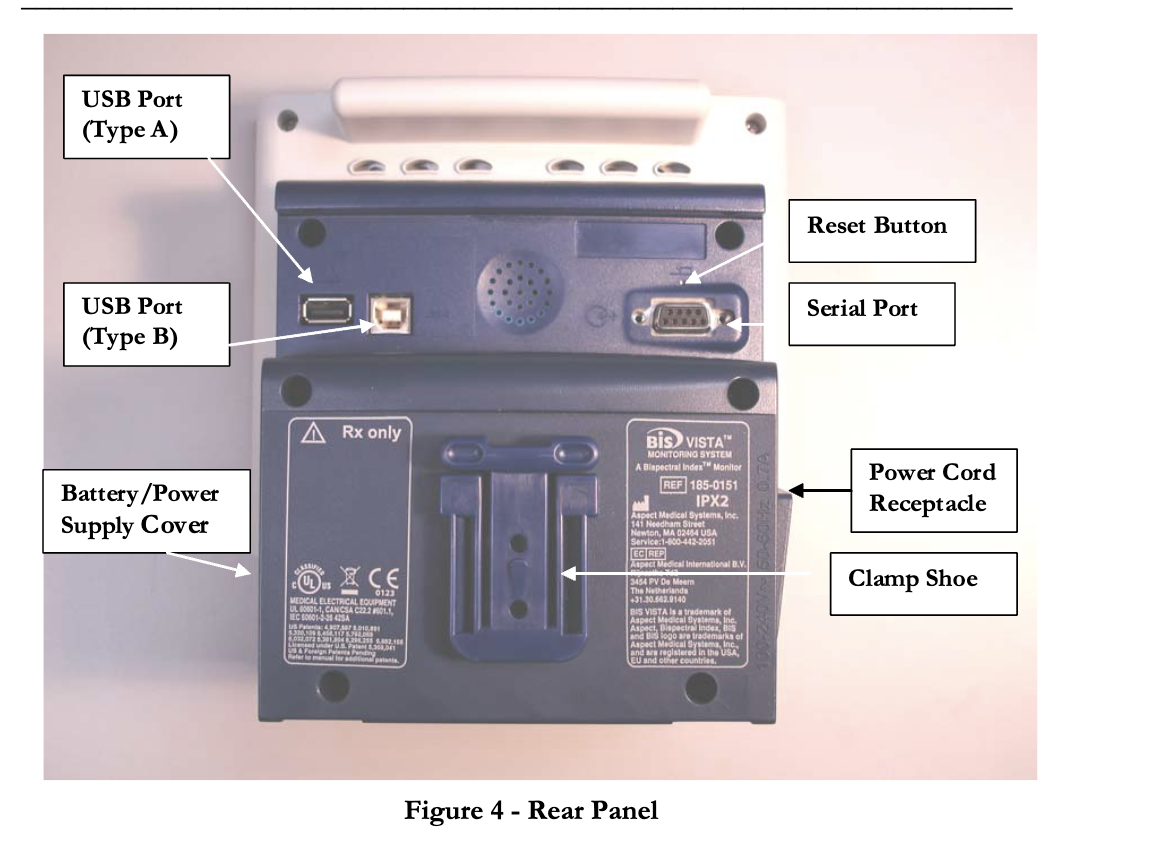
\includegraphics[scale=0.5]{img/bis_rear_panel.png}
    \caption{Caption}
	\label{fig:bis_rear_panel}
\end{figure}


\subsection{Uso}

Después de conectar el cintillo al paciente y esperar a que la señal se estabilice, se debe presionar el botón 'Exportar datos'. A continuación, seleccione la opción 'Datos Activos' y luego elija 'Iniciar exportación'. De esta manera, los datos se guardarán en el pendrive durante la cirugía, permitiendo luego volver a la pantalla principal del monitor.


Clonar el repositorio de Github: \url{https://github.com/cgvalle/monitor_signos_vitales}. En la carpeta \textbf{bis\_record} encontraras dos archivos:

\begin{itemize}
	\item \textbf{main.py}: Este programa se encargara de enviar marcadores al monitor para que se guarden en el pendrive.
	\item \textbf{config.json }: Archivo de configuración que contiene con que tecla se envia el marcador.
	\item \textbf{output.txt} : Archivo donde se guardaran los marcadores enviados.
	\item \textbf{README.md}: Instructivo rapido de uso.
\end{itemize}



Para ejecutar el programa, es necesario abrir una terminal en la carpeta \textbf{bis\_record} y ejecutar el comando \texttt{python main.py}. El programa solicitará que presione la tecla especificada en el archivo de configuración. Cada vez que se presione dicha tecla, se guardará un marcador tanto en el archivo \textbf{output.txt} como en el pendrive. A continuación, se le pedirá que elija el puerto COM al cual está conectado el monitor. Si solo hay un dispositivo conectado, el puerto COM se identificará automáticamente en la lista. De lo contrario, deberá buscarlo manualmente en el Administrador de Dispositivos de Windows.

Para finalizar la adquisición de datos, simplemente cierre la ventana del programa.


\subsection{Resolución de problemas}

A continuación, se presentan soluciones a problemas comunes que pueden surgir al intentar ejecutar el programa:

\begin{itemize}
	\item Si el programa no inicia, asegúrese de haber abierto la carpeta \textbf{bis\_record} en Visual Studio Code y de haber iniciado una terminal en esta misma carpeta.
	\item Si el programa aún no se ejecuta, verifique que el puerto COM seleccionado corresponda al dispositivo conectado. Puede necesitar confirmar el puerto COM a través del Administrador de Dispositivos de Windows.
	\item Si persisten los problemas para ejecutar el programa, asegúrese de que la carpeta \textbf{bis\_record} esté configurada como "confiable" ("trust") dentro de Visual Studio Code. Esto se puede ajustar en las configuraciones de seguridad del entorno de desarrollo.
\end{itemize}












\end{document}
